\clearpage{\pagestyle{empty}\cleardoublepage}

\chapter{Data to Monte Carlo comparison in the preselection region}
\label{app:datamcpresel}

In this appendix more details are given about the 
validation of the modeling of the main backgrounds in
control regions defined at the preselection level 
(see Section~\ref{sec:presel}). A {\it blinding cut}
is defined using the $\htfj$ variable defined as the scalar sum of the
lepton transvers momentum, the first four leading jets transverse momenta
and the missing transverse energy. Considering the typical hardness of
vector-like top partners decay events, the region with $\htfj<800\gev$ can
safely be considered as signal-free. 
%It is worth noticing here that in the $\TTbar\to Wb+X$ analysis this cut is going to be inverted, obtaining an efficient reduction of background contributions, while in the  $\TTbar\to Ht+X$ analysis the  $H_T$ variable (with a slightly different definition, i.e. all jets are included in the sum and not only the first four) is going to be used to discriminate signal and background in the statistical analysis.
The preselection requirement of at least one \bjet\ enriches these control
regions in $\ttbar$+jets background, while  a selection vetoing \bjet s\
is considered to check the modeling of $W$+jets background.
Tables~\ref{tab:yieldspreselELE},~\ref{tab:yieldspreselMUON} and~\ref{tab:yieldspreselELEMUON}
present the yields obtained for data and backgrounds in these two regions,
for electron and muon channels separately and combined.
The following sections show the distributions for some variables of interest
in the same regions again for electron and muon channels separately and combined.

\begin{table}[htb]\centering
%        \resizebox{1.\textwidth}{!}{
        \begin{tabular}{l D{;}{\,\pm\,}{-1} D{;}{\,\pm\,}{-1} } \toprule\toprule
 & \multicolumn{1}{c}{ $\geq 4$ jets, $= 0$ $b$-tags } 		 & \multicolumn{1}{c}{ $\geq 4$ jets, $\geq 1$ $b$-tags } 		 \\ \midrule 
  MultiJet  & 8416;58  & 2524;40 \\ 
 Single top  & 1772;39  & 6615;72 \\ 
 Diboson  & 1006;14  & 246;8 \\ 
 $Z$+jets  & 21287;310  & 3662;111 \\ 
 $W$+jets  & 65702;562  & 14546;312 \\ 
 $t\bar{t}$V  & 51;1  & 303;2 \\ 
 $t\bar{t}$H (125)  & 10;0  & 97;0 \\ 
 $t\bar{t}$ MC@NLO  & 15587;87  & 90839;188 \\ 
\midrule 
  Tot Bkg w/ MC@NLO  & 113831;652  & 118832;390 \\ \midrule 
  $T\bar{T}$ (600) chiral  & 1;0  & 15;1 \\ 
 Data  & 112336;335  & 115175;339 \\ 
\bottomrule\end{tabular}
%}
\caption{Yields for data, backgrounds and signal in the electron channel in the two blinded control
                regions. Uncertainties are only statistical.}\label{tab:yieldspreselELE}
\end{table}

\begin{table}[htb]\centering
%        \resizebox{1.\textwidth}{!}{
        \begin{tabular}{l D{;}{\,\pm\,}{-1} D{;}{\,\pm\,}{-1} } \toprule\toprule
 & \multicolumn{1}{c}{ $\geq 4$ jets, $= 0$ $b$-tags } 		 & \multicolumn{1}{c}{ $\geq 4$ jets, $\geq 1$ $b$-tags } 		 \\ \midrule 
  MultiJet  & 6718;75  & 3740;62 \\ 
 Single top  & 2178;44  & 7760;80 \\ 
 Diboson  & 1166;16  & 302;9 \\ 
 $Z$+jets  & 10115;218  & 2142;95 \\ 
 $W$+jets  & 101849;761  & 21374;423 \\ 
 $t\bar{t}$V  & 62;1  & 377;2 \\ 
 $t\bar{t}$H (125)  & 13;0  & 123;1 \\ 
 $t\bar{t}$ MC@NLO  & 18976;98  & 111202;214 \\ 
\midrule 
  Tot Bkg w/ MC@NLO  & 141076;803  & 147022;494 \\ \midrule 
  $T\bar{T}$ (600) chiral  & 2;1  & 21;2 \\ 
 Data  & 126373;355  & 141818;377 \\ 
\bottomrule\end{tabular}
%}
\caption{Yields for data, backgrounds and signal in the muon  channel in the two blinded control
                regions. Uncertainties are only statistical.}\label{tab:yieldspreselMUON}
\end{table}

\begin{table}[htb]\centering
%        \resizebox{1.\textwidth}{!}{
        \begin{tabular}{l D{;}{\,\pm\,}{-1} D{;}{\,\pm\,}{-1} } \toprule\toprule
 & \multicolumn{1}{c}{ $\geq 4$ jets, $= 0$ $b$-tags } 		 & \multicolumn{1}{c}{ $\geq 4$ jets, $\geq 1$ $b$-tags } 		 \\ \midrule 
  MultiJet  & 15134;95  & 6264;74 \\ 
 Single top  & 3950;59  & 14375;107 \\ 
 Diboson  & 2172;22  & 548;12 \\ 
 $Z$+jets  & 31401;379  & 5804;146 \\ 
 $W$+jets  & 167551;947  & 35921;525 \\ 
 $t\bar{t}$V  & 113;1  & 680;2 \\ 
 $t\bar{t}$H (125)  & 24;0  & 220;1 \\ 
 $t\bar{t}$ MC@NLO  & 34563;131  & 202042;285 \\ 
\midrule 
  Tot Bkg w/ MC@NLO  & 254907;1034  & 265854;629 \\ \midrule 
  $T\bar{T}$ (600) chiral  & 3;1  & 36;2 \\ 
 Data  & 238709;489  & 256993;507 \\ 
\bottomrule\end{tabular}
%}
\caption{Yields for data, backgrounds and signal in the combined electron+muon  channel in the two blinded control
                regions. Uncertainties are only statistical.}\label{tab:yieldspreselELEMUON}
\end{table}



\clearpage 

\section{Data to Monte Carlo comparison vetoing \bjet s}
\label{app:datamc0tagex}

\subsection{Electron channel}

\begin{figure}[h!]\begin{center}
	\subfigure[]{
  	\includegraphics[width=0.29\textwidth]{vlq_analysis/figures/THESIS_c5_presel_noortho_noyields/ELE/4jetin/0btagex/Njets25_ELE_4jetin0btagex_NOMINAL}}
	\subfigure[]{
  	\includegraphics[width=0.29\textwidth]{vlq_analysis/figures/THESIS_c5_presel_noortho_noyields/ELE/4jetin/0btagex/JetPt1_ELE_4jetin0btagex_NOMINAL}}
	\subfigure[]{
  	\includegraphics[width=0.29\textwidth]{vlq_analysis/figures/THESIS_c5_presel_noortho_noyields/ELE/4jetin/0btagex/JetEta1_ELE_4jetin0btagex_NOMINAL}}\\
	\subfigure[]{
  	\includegraphics[width=0.29\textwidth]{vlq_analysis/figures/THESIS_c5_presel_noortho_noyields/ELE/4jetin/0btagex/MET_ELE_4jetin0btagex_NOMINAL}}
	\subfigure[]{
  	\includegraphics[width=0.29\textwidth]{vlq_analysis/figures/THESIS_c5_presel_noortho_noyields/ELE/4jetin/0btagex/LepPt_ELE_4jetin0btagex_NOMINAL}}
	\subfigure[]{
  	\includegraphics[width=0.29\textwidth]{vlq_analysis/figures/THESIS_c5_presel_noortho_noyields/ELE/4jetin/0btagex/LepEta_ELE_4jetin0btagex_NOMINAL}}\\
	\subfigure[]{
  	\includegraphics[width=0.29\textwidth]{vlq_analysis/figures/THESIS_c5_presel_noortho_noyields/ELE/4jetin/0btagex/Wlep_MassT_ELE_4jetin0btagex_NOMINAL}}
	\subfigure[]{
  	\includegraphics[width=0.29\textwidth]{vlq_analysis/figures/THESIS_c5_presel_noortho_noyields/ELE/4jetin/0btagex/HTHad_ELE_4jetin0btagex_NOMINAL}}
	\subfigure[]{
  	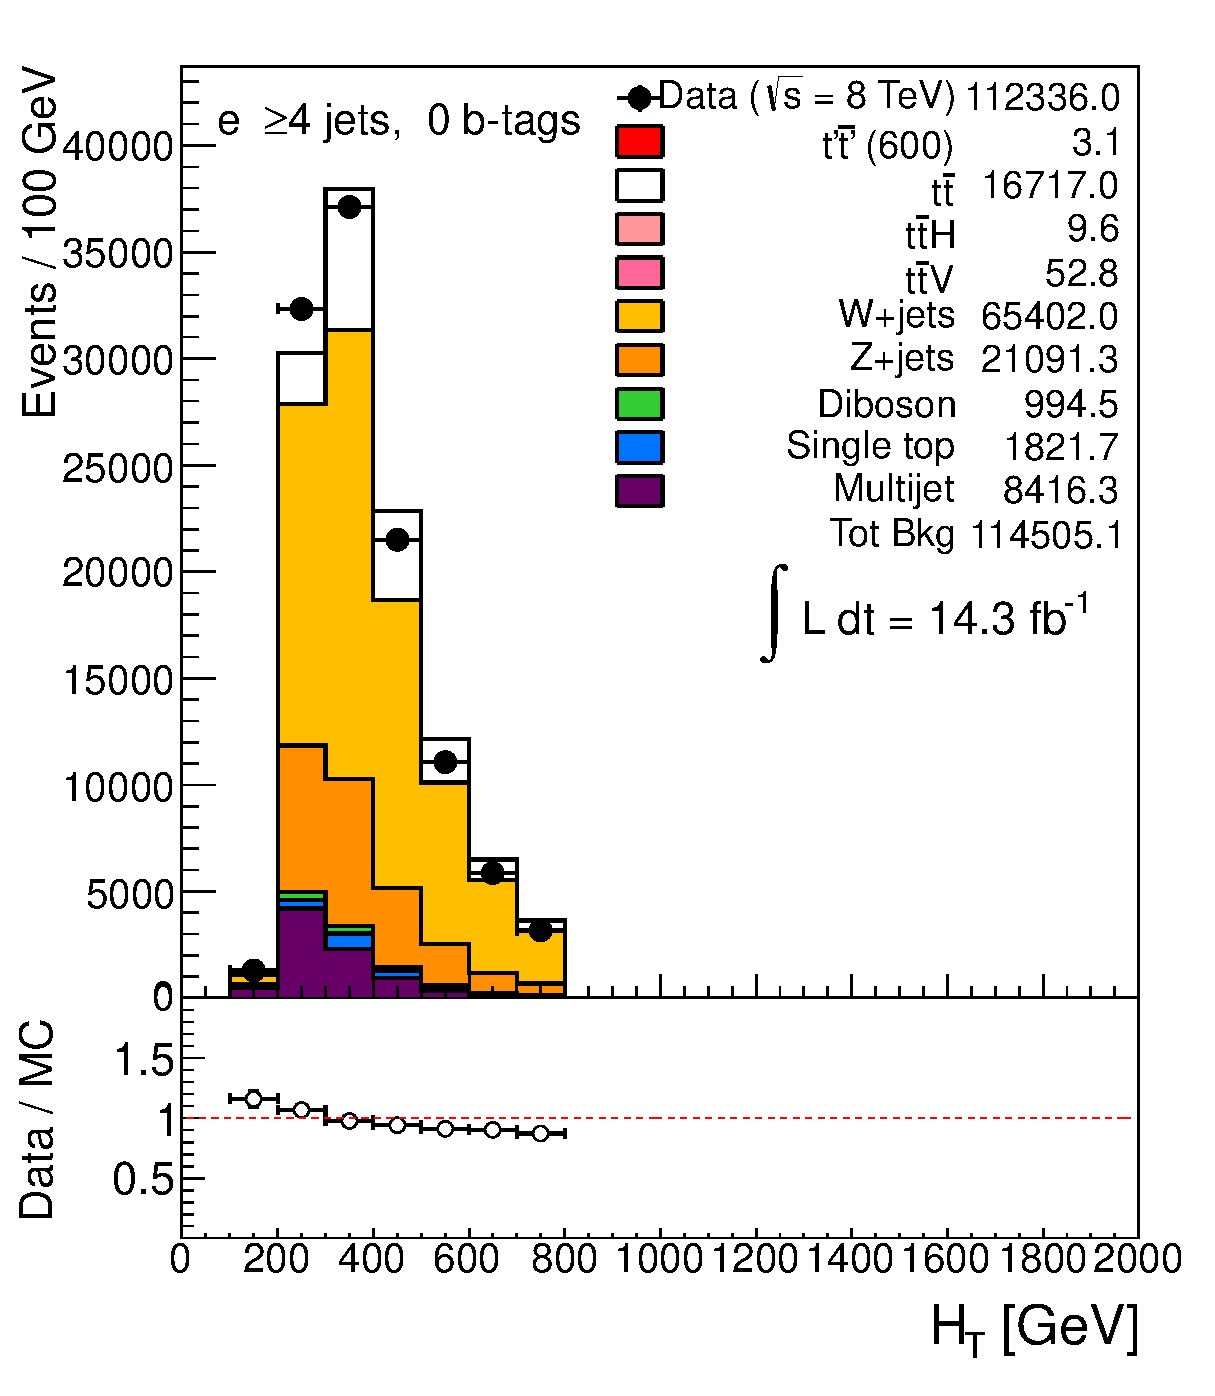
\includegraphics[width=0.29\textwidth]{vlq_analysis/figures/THESIS_c5_presel_noortho_noyields/ELE/4jetin/0btagex/HTAll_ELE_4jetin0btagex_NOMINAL}}
	\caption[]{Comparison between data and prediction in the
        electron
        channel in the blinded control region with at least four jets and
        no \bjet s
        \input{appendices/datamc_variablelist.tex}
         \label{fig:appELE_4jetin0btagex}}
\end{center}\end{figure}


\clearpage
\subsection{Muon channel}


\begin{figure}[h!]\begin{center}
	\subfigure[]{
  	\includegraphics[width=0.29\textwidth]{vlq_analysis/figures/THESIS_c5_presel_noortho_noyields/MUON/4jetin/0btagex/Njets25_MUON_4jetin0btagex_NOMINAL}}
	\subfigure[]{
  	\includegraphics[width=0.29\textwidth]{vlq_analysis/figures/THESIS_c5_presel_noortho_noyields/MUON/4jetin/0btagex/JetPt1_MUON_4jetin0btagex_NOMINAL}}
	\subfigure[]{
  	\includegraphics[width=0.29\textwidth]{vlq_analysis/figures/THESIS_c5_presel_noortho_noyields/MUON/4jetin/0btagex/JetEta1_MUON_4jetin0btagex_NOMINAL}}\\
	\subfigure[]{
  	\includegraphics[width=0.29\textwidth]{vlq_analysis/figures/THESIS_c5_presel_noortho_noyields/MUON/4jetin/0btagex/MET_MUON_4jetin0btagex_NOMINAL}}
	\subfigure[]{
  	\includegraphics[width=0.29\textwidth]{vlq_analysis/figures/THESIS_c5_presel_noortho_noyields/MUON/4jetin/0btagex/LepPt_MUON_4jetin0btagex_NOMINAL}}
	\subfigure[]{
  	\includegraphics[width=0.29\textwidth]{vlq_analysis/figures/THESIS_c5_presel_noortho_noyields/MUON/4jetin/0btagex/LepEta_MUON_4jetin0btagex_NOMINAL}}\\
	\subfigure[]{
  	\includegraphics[width=0.29\textwidth]{vlq_analysis/figures/THESIS_c5_presel_noortho_noyields/MUON/4jetin/0btagex/Wlep_MassT_MUON_4jetin0btagex_NOMINAL}}
	\subfigure[]{
  	\includegraphics[width=0.29\textwidth]{vlq_analysis/figures/THESIS_c5_presel_noortho_noyields/MUON/4jetin/0btagex/HTHad_MUON_4jetin0btagex_NOMINAL}}
	\subfigure[]{
  	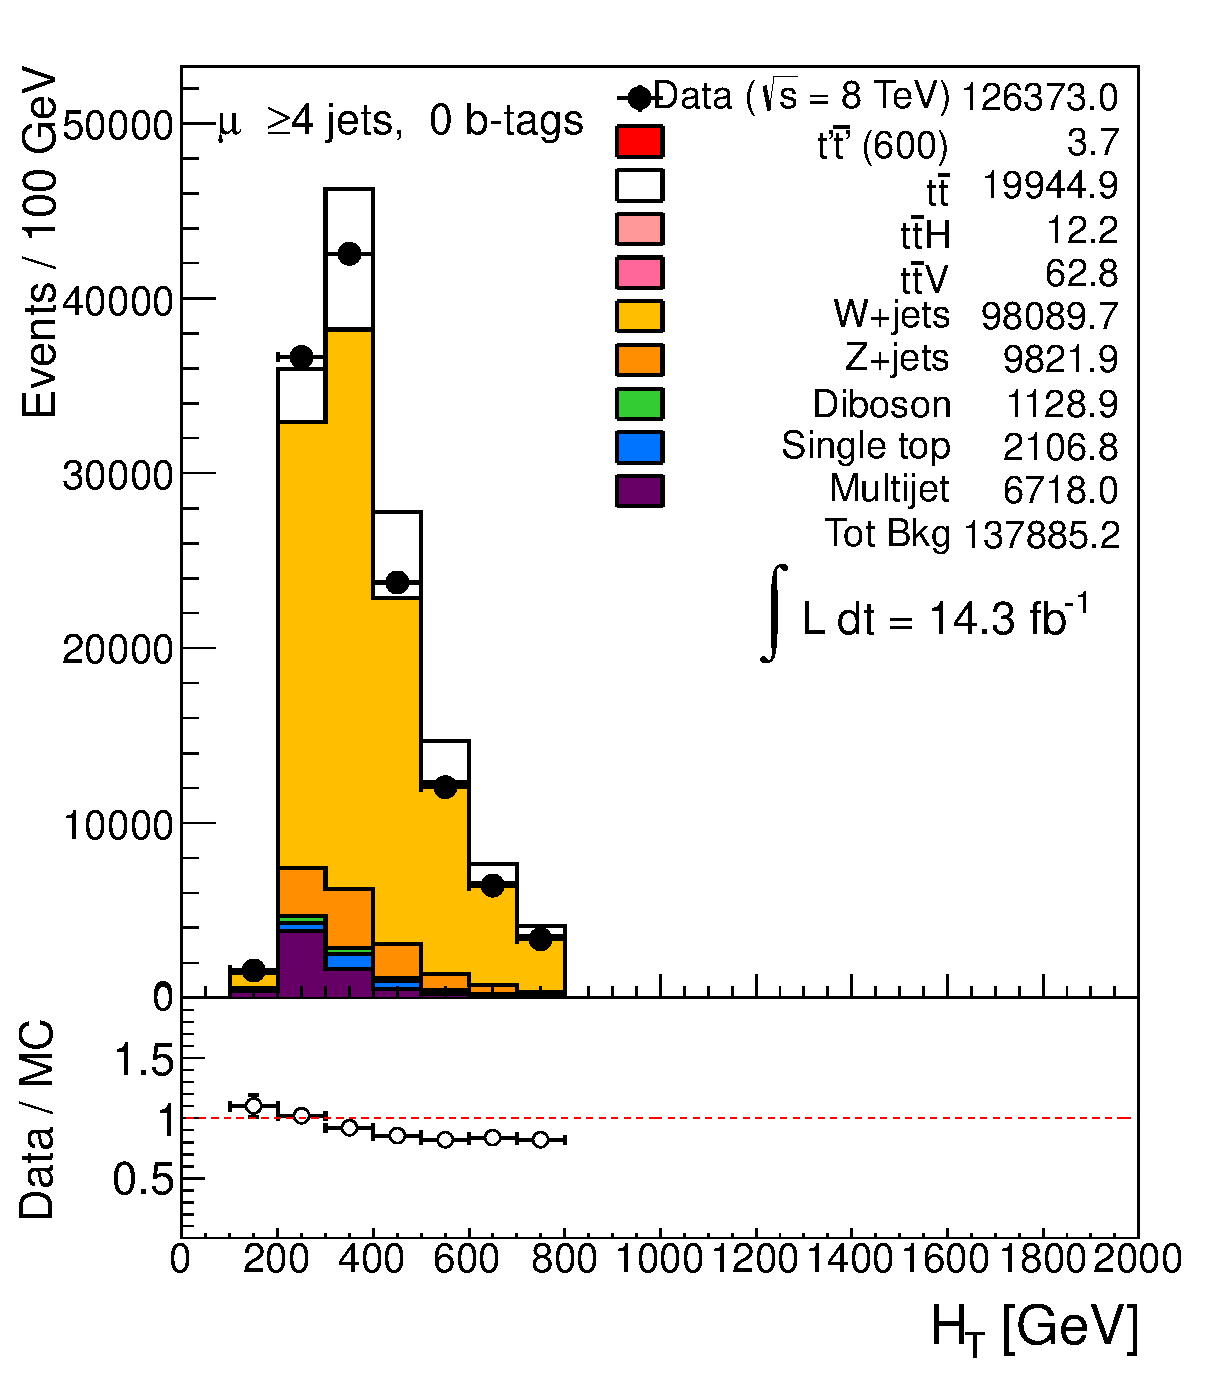
\includegraphics[width=0.29\textwidth]{vlq_analysis/figures/THESIS_c5_presel_noortho_noyields/MUON/4jetin/0btagex/HTAll_MUON_4jetin0btagex_NOMINAL}}
	\caption[]{Comparison between data and prediction in the
        muon 
        channel in the blinded control region with at least four jets and
        no \bjet s
        \input{appendices/datamc_variablelist.tex}
	\label{fig:appMUON_4jetin0btagex}}
\end{center}\end{figure}


\clearpage
\subsection{Electron+Muon channel}

\begin{figure}[h!]\begin{center}
	\subfigure[]{
  	\includegraphics[width=0.29\textwidth]{vlq_analysis/figures/THESIS_c5_presel_noortho_noyields/ELEMUON/4jetin/0btagex/Njets25_ELEMUON_4jetin0btagex_NOMINAL}}
	\subfigure[]{
  	\includegraphics[width=0.29\textwidth]{vlq_analysis/figures/THESIS_c5_presel_noortho_noyields/ELEMUON/4jetin/0btagex/JetPt1_ELEMUON_4jetin0btagex_NOMINAL}}
	\subfigure[]{
  	\includegraphics[width=0.29\textwidth]{vlq_analysis/figures/THESIS_c5_presel_noortho_noyields/ELEMUON/4jetin/0btagex/JetEta1_ELEMUON_4jetin0btagex_NOMINAL}}\\
	\subfigure[]{
  	\includegraphics[width=0.29\textwidth]{vlq_analysis/figures/THESIS_c5_presel_noortho_noyields/ELEMUON/4jetin/0btagex/MET_ELEMUON_4jetin0btagex_NOMINAL}}
	\subfigure[]{
  	\includegraphics[width=0.29\textwidth]{vlq_analysis/figures/THESIS_c5_presel_noortho_noyields/ELEMUON/4jetin/0btagex/LepPt_ELEMUON_4jetin0btagex_NOMINAL}}
	\subfigure[]{
  	\includegraphics[width=0.29\textwidth]{vlq_analysis/figures/THESIS_c5_presel_noortho_noyields/ELEMUON/4jetin/0btagex/LepEta_ELEMUON_4jetin0btagex_NOMINAL}}\\
	\subfigure[]{
  	\includegraphics[width=0.29\textwidth]{vlq_analysis/figures/THESIS_c5_presel_noortho_noyields/ELEMUON/4jetin/0btagex/Wlep_MassT_ELEMUON_4jetin0btagex_NOMINAL}}
	\subfigure[]{
  	\includegraphics[width=0.29\textwidth]{vlq_analysis/figures/THESIS_c5_presel_noortho_noyields/ELEMUON/4jetin/0btagex/HTHad_ELEMUON_4jetin0btagex_NOMINAL}}
	\subfigure[]{
  	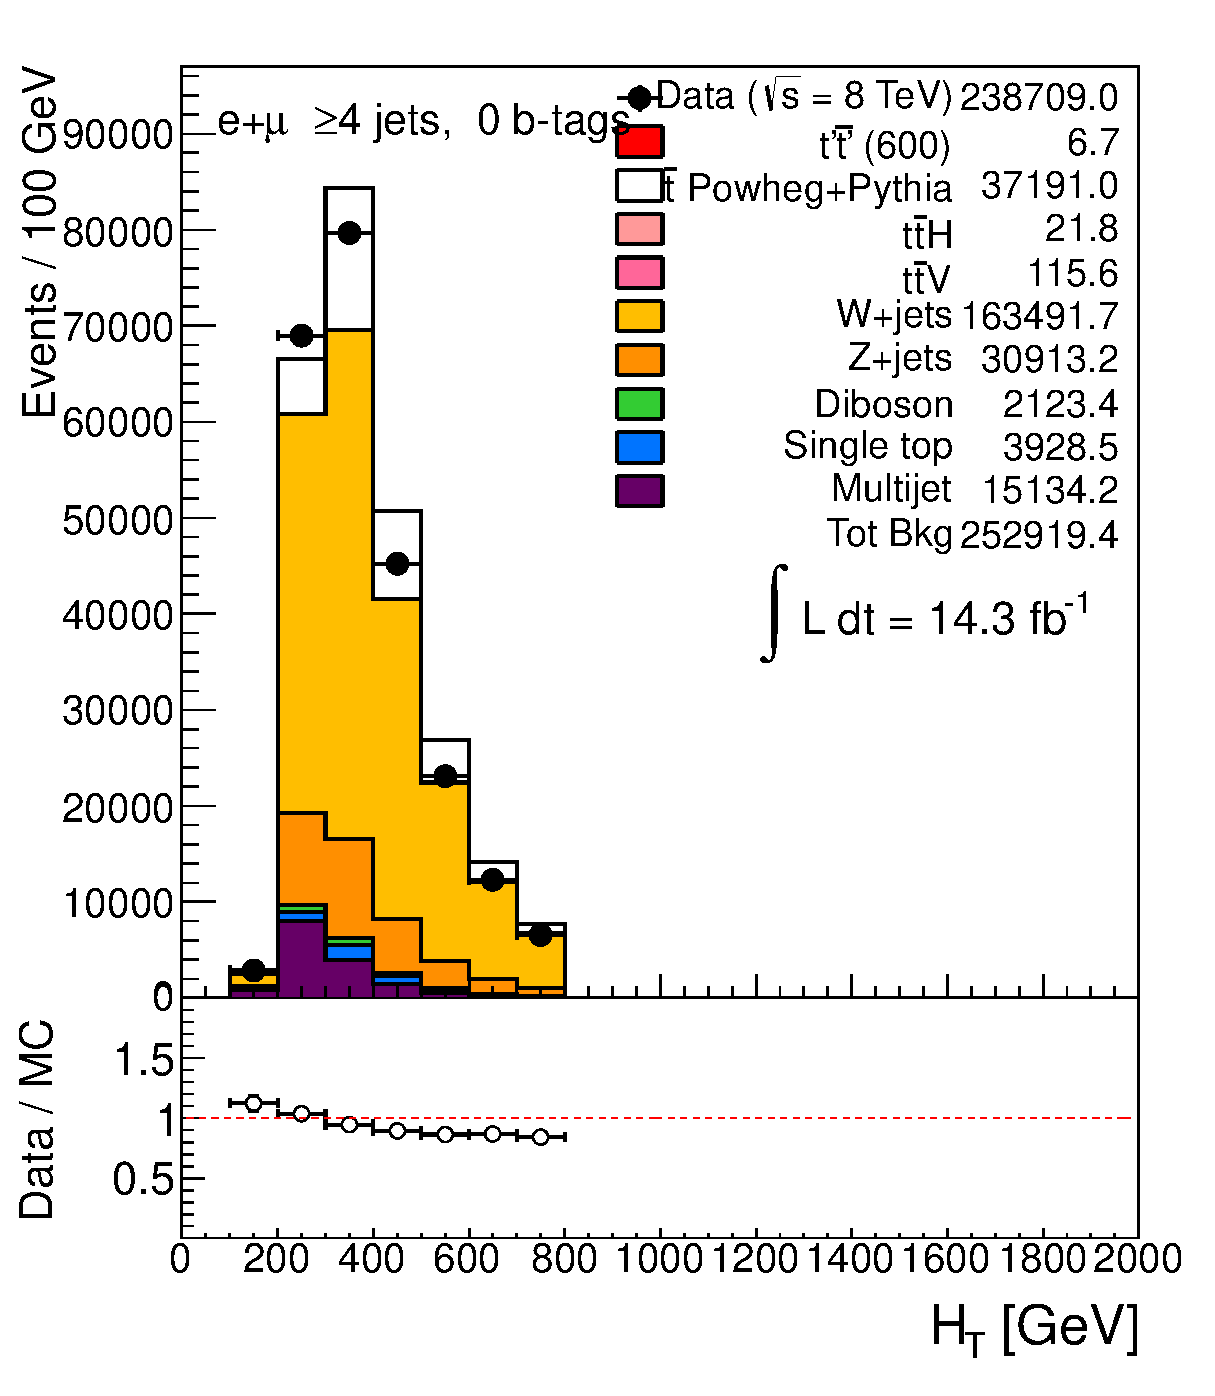
\includegraphics[width=0.29\textwidth]{vlq_analysis/figures/THESIS_c5_presel_noortho_noyields/ELEMUON/4jetin/0btagex/HTAll_ELEMUON_4jetin0btagex_NOMINAL}}
	\caption[]{Comparison between data and prediction in the
        combined electron and muon 
        channel in the blinded control region with at least four jets and
        no \bjet s
        \input{appendices/datamc_variablelist.tex}
	\label{fig:appELEMUON_4jetin0btagex}}
\end{center}\end{figure}



\section{Comparison between data and prediction requiring at least 1 \bjet}
\label{app:datamc1tagin}



\subsection{Electron channel}

\begin{figure}[h!]\begin{center}
	\subfigure[]{
  	\includegraphics[width=0.29\textwidth]{vlq_analysis/figures/THESIS_c5_presel_noortho_noyields/ELE/4jetin/1btagin/Njets25_ELE_4jetin1btagin_NOMINAL}}
	\subfigure[]{
  	\includegraphics[width=0.29\textwidth]{vlq_analysis/figures/THESIS_c5_presel_noortho_noyields/ELE/4jetin/1btagin/JetPt1_ELE_4jetin1btagin_NOMINAL}}
	\subfigure[]{
  	\includegraphics[width=0.29\textwidth]{vlq_analysis/figures/THESIS_c5_presel_noortho_noyields/ELE/4jetin/1btagin/JetEta1_ELE_4jetin1btagin_NOMINAL}}\\
	\subfigure[]{
  	\includegraphics[width=0.29\textwidth]{vlq_analysis/figures/THESIS_c5_presel_noortho_noyields/ELE/4jetin/1btagin/MET_ELE_4jetin1btagin_NOMINAL}}
	\subfigure[]{
  	\includegraphics[width=0.29\textwidth]{vlq_analysis/figures/THESIS_c5_presel_noortho_noyields/ELE/4jetin/1btagin/LepPt_ELE_4jetin1btagin_NOMINAL}}
	\subfigure[]{
  	\includegraphics[width=0.29\textwidth]{vlq_analysis/figures/THESIS_c5_presel_noortho_noyields/ELE/4jetin/1btagin/LepEta_ELE_4jetin1btagin_NOMINAL}}\\
	\subfigure[]{
  	\includegraphics[width=0.29\textwidth]{vlq_analysis/figures/THESIS_c5_presel_noortho_noyields/ELE/4jetin/1btagin/Wlep_MassT_ELE_4jetin1btagin_NOMINAL}}
	\subfigure[]{
  	\includegraphics[width=0.29\textwidth]{vlq_analysis/figures/THESIS_c5_presel_noortho_noyields/ELE/4jetin/1btagin/HTHad_ELE_4jetin1btagin_NOMINAL}}
	\subfigure[]{
  	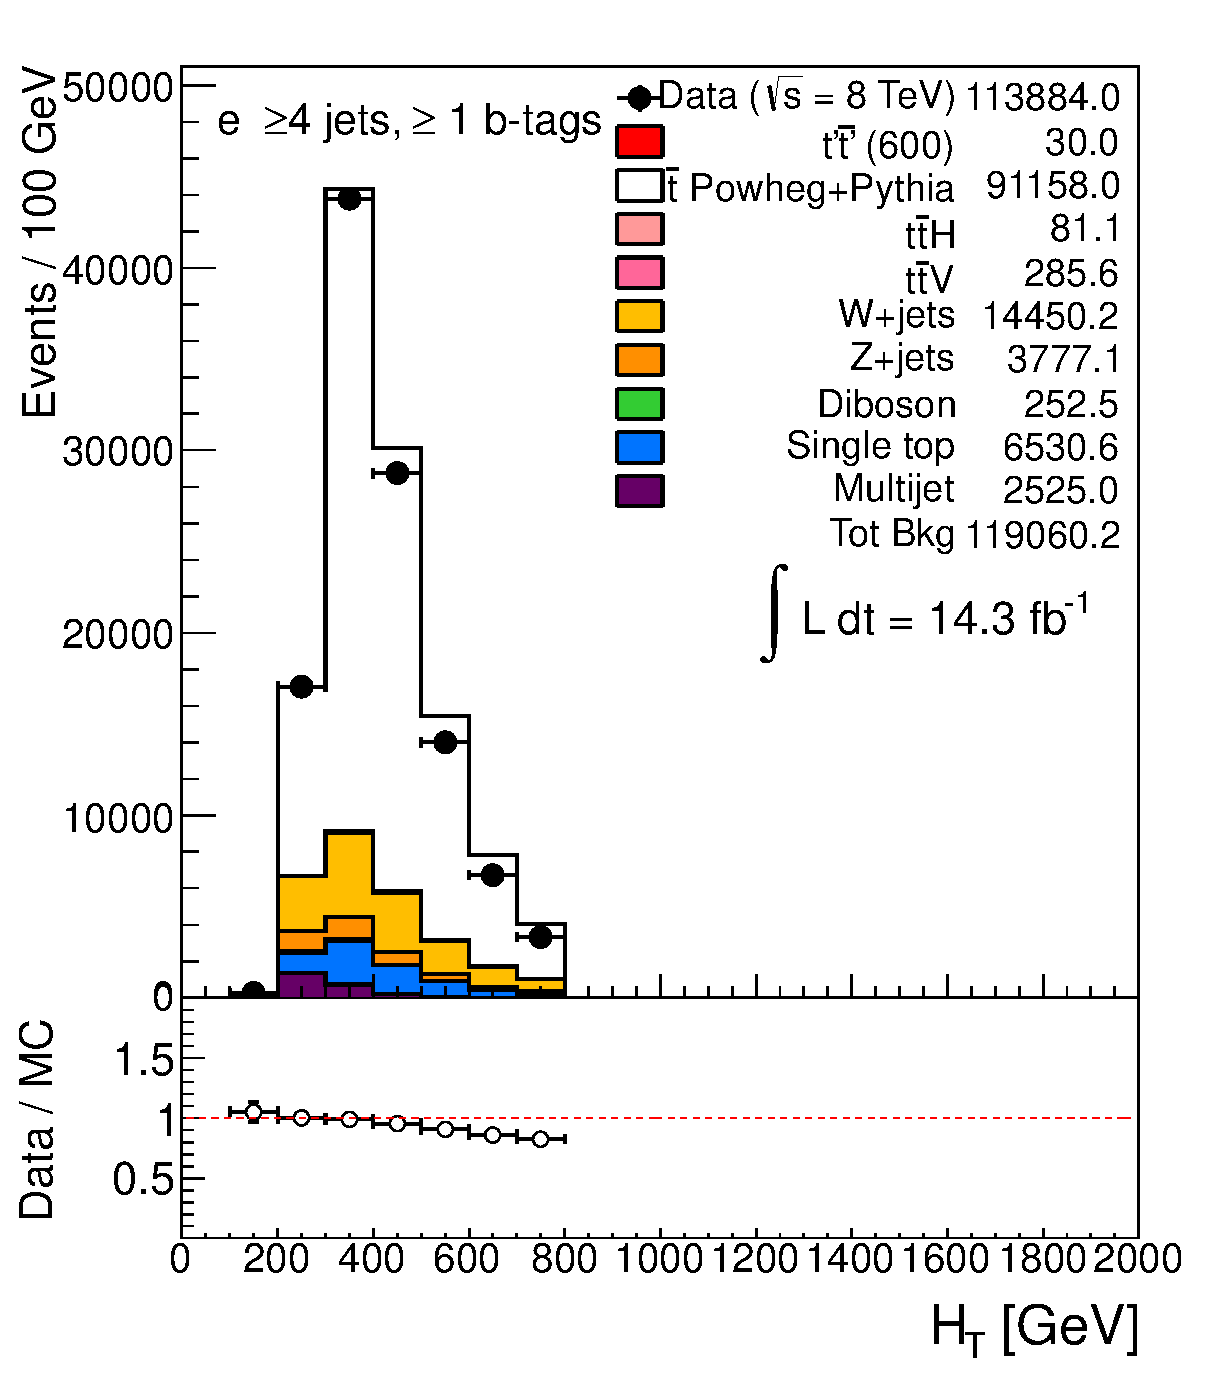
\includegraphics[width=0.29\textwidth]{vlq_analysis/figures/THESIS_c5_presel_noortho_noyields/ELE/4jetin/1btagin/HTAll_ELE_4jetin1btagin_NOMINAL}}
	\caption[]{Comparison between data and prediction in the
        electron
        channel in the blinded control region with at least four jets and
        no \bjet s
        \input{appendices/datamc_variablelist.tex}
         \label{fig:appELE_4jetin1btagin}}
\end{center}\end{figure}


\clearpage
\subsection{Muon channel}


\begin{figure}[h!]\begin{center}
	\subfigure[]{
  	\includegraphics[width=0.29\textwidth]{vlq_analysis/figures/THESIS_c5_presel_noortho_noyields/MUON/4jetin/1btagin/Njets25_MUON_4jetin1btagin_NOMINAL}}
	\subfigure[]{
  	\includegraphics[width=0.29\textwidth]{vlq_analysis/figures/THESIS_c5_presel_noortho_noyields/MUON/4jetin/1btagin/JetPt1_MUON_4jetin1btagin_NOMINAL}}
	\subfigure[]{
  	\includegraphics[width=0.29\textwidth]{vlq_analysis/figures/THESIS_c5_presel_noortho_noyields/MUON/4jetin/1btagin/JetEta1_MUON_4jetin1btagin_NOMINAL}}\\
	\subfigure[]{
  	\includegraphics[width=0.29\textwidth]{vlq_analysis/figures/THESIS_c5_presel_noortho_noyields/MUON/4jetin/1btagin/MET_MUON_4jetin1btagin_NOMINAL}}
	\subfigure[]{
  	\includegraphics[width=0.29\textwidth]{vlq_analysis/figures/THESIS_c5_presel_noortho_noyields/MUON/4jetin/1btagin/LepPt_MUON_4jetin1btagin_NOMINAL}}
	\subfigure[]{
  	\includegraphics[width=0.29\textwidth]{vlq_analysis/figures/THESIS_c5_presel_noortho_noyields/MUON/4jetin/1btagin/LepEta_MUON_4jetin1btagin_NOMINAL}}\\
	\subfigure[]{
  	\includegraphics[width=0.29\textwidth]{vlq_analysis/figures/THESIS_c5_presel_noortho_noyields/MUON/4jetin/1btagin/Wlep_MassT_MUON_4jetin1btagin_NOMINAL}}
	\subfigure[]{
  	\includegraphics[width=0.29\textwidth]{vlq_analysis/figures/THESIS_c5_presel_noortho_noyields/MUON/4jetin/1btagin/HTHad_MUON_4jetin1btagin_NOMINAL}}
	\subfigure[]{
  	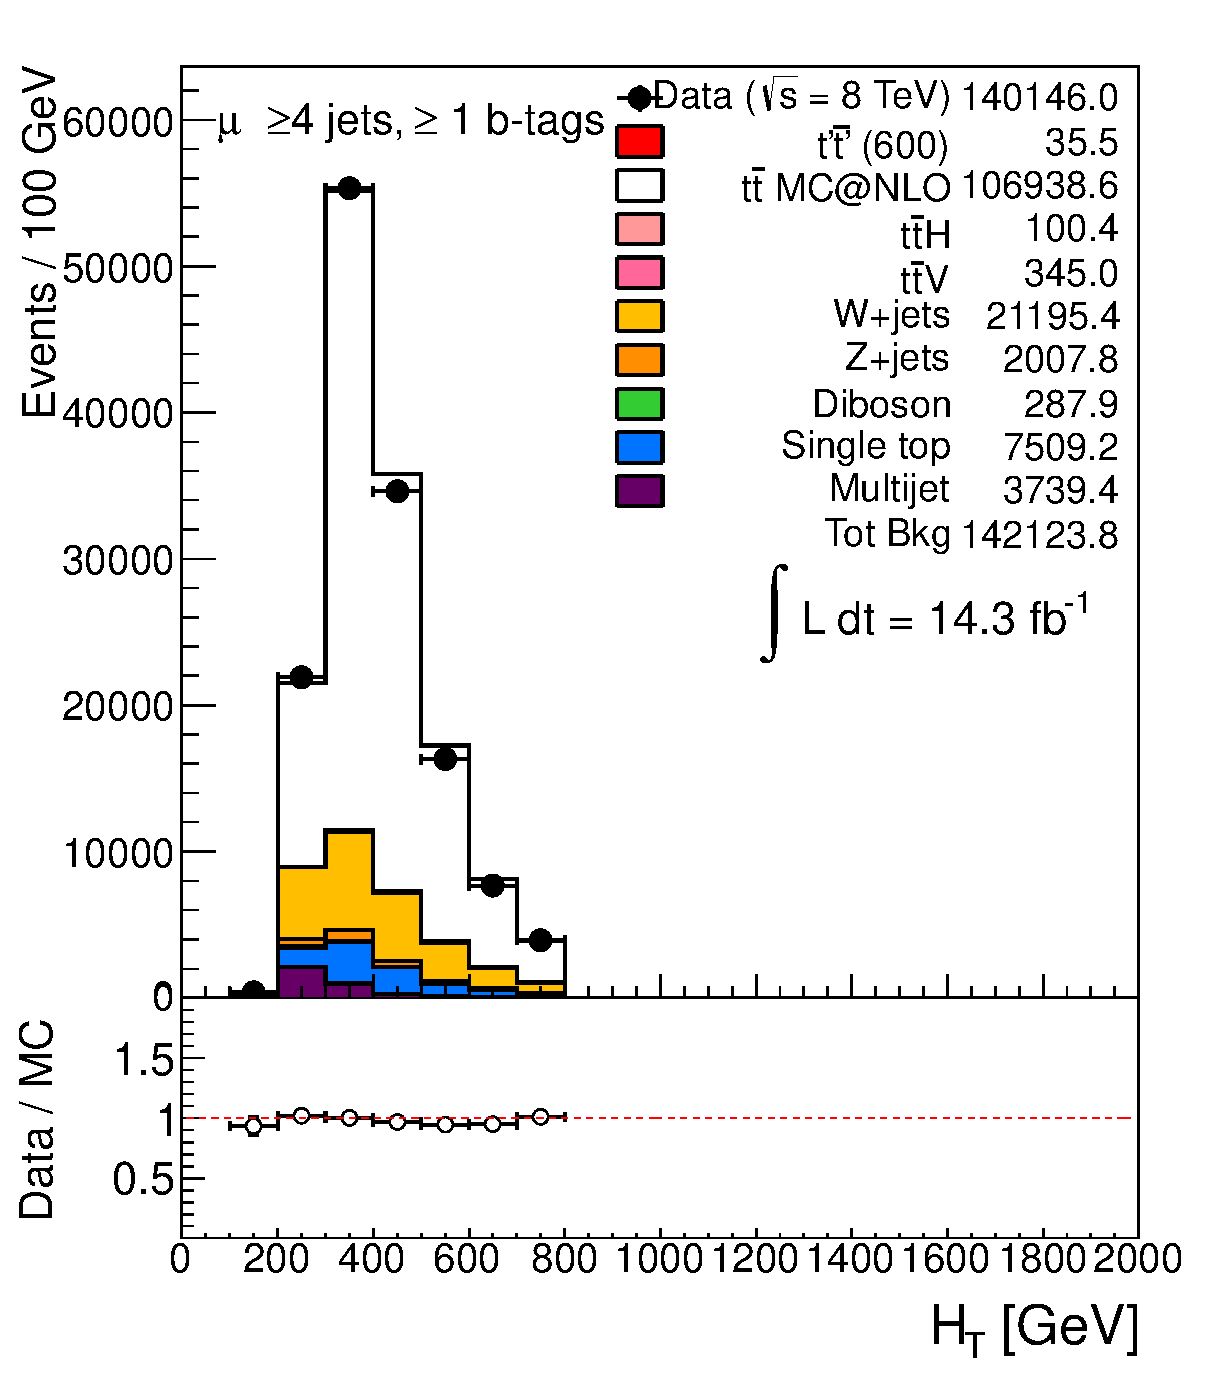
\includegraphics[width=0.29\textwidth]{vlq_analysis/figures/THESIS_c5_presel_noortho_noyields/MUON/4jetin/1btagin/HTAll_MUON_4jetin1btagin_NOMINAL}}
	\caption[]{Comparison between data and prediction in the
        muon 
        channel in the blinded control region with at least four jets and
        no \bjet s
        \input{appendices/datamc_variablelist.tex}
	\label{fig:appMUON_4jetin1btagin}}
\end{center}\end{figure}


\clearpage
\subsection{Electron and muon combined channel}

\begin{figure}[h!]\begin{center}
	\subfigure[]{
  	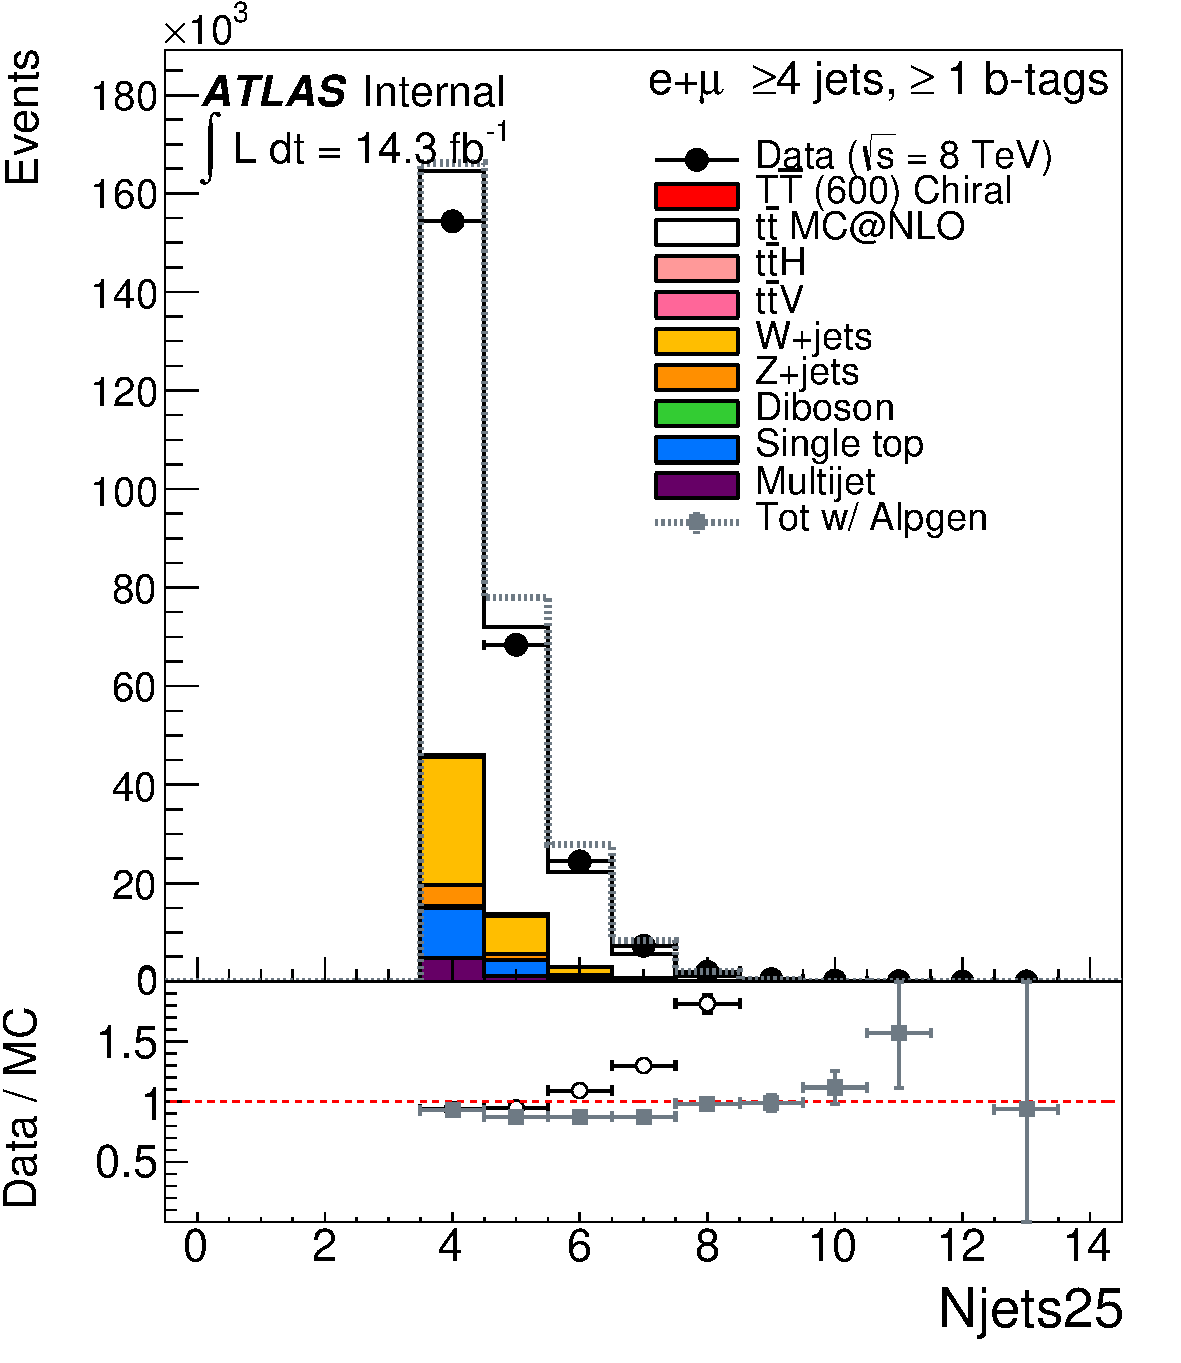
\includegraphics[width=0.29\textwidth]{vlq_analysis/figures/THESIS_c5_presel_noortho_noyields/ELEMUON/4jetin/1btagin/Njets25_ELEMUON_4jetin1btagin_NOMINAL}}
	\subfigure[]{
  	\includegraphics[width=0.29\textwidth]{vlq_analysis/figures/THESIS_c5_presel_noortho_noyields/ELEMUON/4jetin/1btagin/JetPt1_ELEMUON_4jetin1btagin_NOMINAL}}
	\subfigure[]{
  	\includegraphics[width=0.29\textwidth]{vlq_analysis/figures/THESIS_c5_presel_noortho_noyields/ELEMUON/4jetin/1btagin/JetEta1_ELEMUON_4jetin1btagin_NOMINAL}}\\
	\subfigure[]{
  	\includegraphics[width=0.29\textwidth]{vlq_analysis/figures/THESIS_c5_presel_noortho_noyields/ELEMUON/4jetin/1btagin/MET_ELEMUON_4jetin1btagin_NOMINAL}}
	\subfigure[]{
  	\includegraphics[width=0.29\textwidth]{vlq_analysis/figures/THESIS_c5_presel_noortho_noyields/ELEMUON/4jetin/1btagin/LepPt_ELEMUON_4jetin1btagin_NOMINAL}}
	\subfigure[]{
  	\includegraphics[width=0.29\textwidth]{vlq_analysis/figures/THESIS_c5_presel_noortho_noyields/ELEMUON/4jetin/1btagin/LepEta_ELEMUON_4jetin1btagin_NOMINAL}}\\
	\subfigure[]{
  	\includegraphics[width=0.29\textwidth]{vlq_analysis/figures/THESIS_c5_presel_noortho_noyields/ELEMUON/4jetin/1btagin/Wlep_MassT_ELEMUON_4jetin1btagin_NOMINAL}}
	\subfigure[]{
  	\includegraphics[width=0.29\textwidth]{vlq_analysis/figures/THESIS_c5_presel_noortho_noyields/ELEMUON/4jetin/1btagin/HTHad_ELEMUON_4jetin1btagin_NOMINAL}}
	\subfigure[]{
  	\includegraphics[width=0.29\textwidth]{vlq_analysis/figures/THESIS_c5_presel_noortho_noyields/ELEMUON/4jetin/1btagin/HTAll_ELEMUON_4jetin1btagin_NOMINAL}}
	\caption[]{Comparison between data and prediction in the
        combined electron and muon 
        channel in the blinded control region with at least four jets and
        no \bjet s
        \input{appendices/datamc_variablelist.tex}
	\label{fig:appELEMUON_4jetin1btagin}}
\end{center}\end{figure}


